% Section content template for individual Educative lessons
% This file contains the actual content for a specific section
% Generated from Educative API section content

% Section: Design of a Code Deployment System
% Section ID: 4940491583782912
% Section Slug: design-of-a-code-deployment-system
% Generated: 2025-12-08T15:28:28.300477

The previous lesson covered the fundamentals of the code deployment system: its requirements, resources, and key components. Now , let's examine the high-level design of the code deployment system.

\subsection{High-level design}\label{pkJ19vNvpHC3_5HSovmfg}
\\
The high-level design of the code deployment system shows the various components we identified in the previous lesson. We have started developing a solution to meet the functional and non-functional requirements with the following design:

\begin{figure}[htbp]
 \centering
 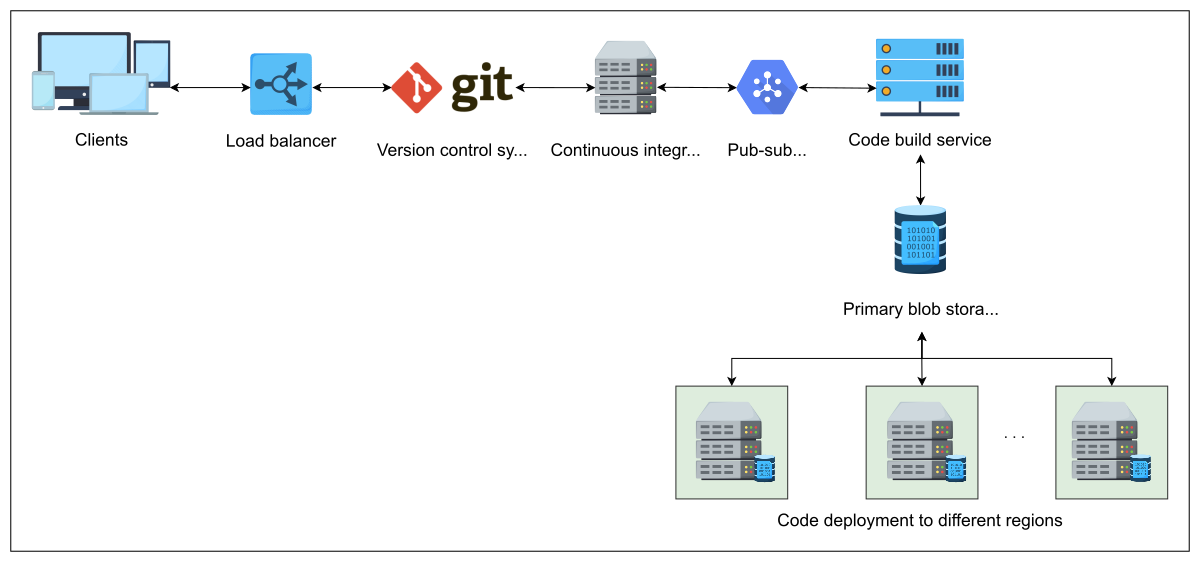
\includegraphics[width=0.5\textwidth]{Images/chapter_39/section_4940491583782912/5711060960935936.png}
 \caption{High-level design of the code deployment system}
\end{figure}

The workflow of the high-level design is shown below:

\begin{itemize}
\item
\protect\phantomsection\label{JcocBnNBXK63yly13A0I_}
Initially, users submit code to the version control system (VCS)(Tool for managing and tracking code changes across versions).
\item
\protect\phantomsection\label{1xSJ-gkU_F3wmNvXOjunc}
The VCS triggers the Continuous Integration (CI(Platform that automatically builds and tests code changes after each commit)) service upon code changes. The CI system automates the process of integrating code changes from multiple developers into a shared repository.
\item
\protect\phantomsection\label{YWJNoPOkuIvyCLc0fvCIo}
The code to build is placed in the pub-sub system. The code-build service takes code from the queue and converts it into a binary.
\item
\protect\phantomsection\label{Z87k0nrSjLn3Fk7lhvD2a}
The generated artifacts (binaries) are stored in the primary blob storage.
\item
\protect\phantomsection\label{xsE3FAC6nrbCA5WRDcCAQ}
Upon initiating deployment, the artifacts (binaries) from the blob storage are downloaded and installed on each machine in each region.
\end{itemize}
\\
To better understand how the system operates at a functional level, let's explore the API design next.

\subsection{API design}\label{qPZaz-Fdw6nmvE7GVJNP1}
\\
The following are essential APIs required for the code-building and deployment process:

\subsubsection{Code-build APIs}\label{tu2Y_kDFm8OFpRfTFVdIy}
\\
Let's discuss some of the important APIs for the code-build process below:

\begin{itemize}
\item
\protect\phantomsection\label{H99SgjZd7sTBdAZhFfOKq}
\textbf{Submit code:} This API is used to submit code to a specified repository in the VCS.
\end{itemize}

\begin{lstlisting}[language=c++17]
submitCode(code, repository, branch, message)
\end{lstlisting}

The \texttt{submitCode()} returns the commit hash uniquely identifying the new commit within the specified repository. This commit hash is used to reference and retrieve the commit later.\\
The following parameters are used for this API:

\begin{table}[htbp]
\centering
\small
\adjustbox{max width=\textwidth}{
\begin{tabular}{|p{0.284\textwidth}|p{0.666\textwidth}|}
\hline
\textbf{Parameter} & \textbf{Description} \\
\hline
\hline
\texttt{code} & The code submitted to the VCS. \\
\hline
\texttt{repository} & This shows a path to a repository where the code is being submitted. \\
\hline
\texttt{branch} & Within a VCS, a branch represents an independent instance of the primary code or repository, typically identified by a unique name. In our case, it shows the branch name where the code is submitted or edited. \\
\hline
\texttt{message} & An optional message during a commit. \\
\hline
\end{tabular}
}
\end{table}

\begin{itemize}
\item
\protect\phantomsection\label{5ASaQQLjLogHkfHrKcqsc}
\textbf{Trigger build:} This API triggers the process of building and preparing the codebase for deployment.\\
\end{itemize}

\begin{lstlisting}[language=c++17]
triggerBuild(project_id, branch, commit_hash, configuration)
\end{lstlisting}

The \texttt{triggerBuild()} API initiates the build process asynchronously. So , this API returns without waiting for the build process to complete. It returns a JSON object containing the URL to the queue where it is placed, and the build\_id assigned to the build.

\begin{table}[htbp]
\centering
\small
\adjustbox{max width=\textwidth}{
\begin{tabular}{|p{0.284\textwidth}|p{0.666\textwidth}|}
\hline
\textbf{Parameter} & \textbf{Description} \\
\hline
\hline
\texttt{project\_id} & The ID of the project for which the build is being triggered. \\
\hline
\texttt{branch} & The branch name where the code is submitted. \\
\hline
\texttt{commit\_hash} & A fixed-length hash value generated using SHA. \\
\hline
\texttt{configuration} & The specific settings, options, parameters, and environment variables that steer the course of the build process. \\
\hline
\end{tabular}
}
\end{table}

\begin{itemize}
\item
\protect\phantomsection\label{ugOucfcP33fw4ptV-M1Bt}
\textbf{Access build artifacts:} This API is used to access the artifacts generated due to the build process.
\end{itemize}

\begin{lstlisting}[language=c++17]
accessBuildArtifacts(build_id)
\end{lstlisting}

\begin{table}[htbp]
\centering
\small
\adjustbox{max width=\textwidth}{
\begin{tabular}{|p{0.284\textwidth}|p{0.666\textwidth}|}
\hline
\textbf{Parameter} & \textbf{Description} \\
\hline
\hline
\texttt{build\_id} & A unique ID assigned to each build. \\
\hline
\end{tabular}
}
\end{table}

\begin{itemize}
\item
\protect\phantomsection\label{hbnDp2mQ82C_Ly60rMV4v}
\textbf{Debug build failures:} This API is used to troubleshoot and fix failures during the build process. When we call this API, it triggers a series of actions or processes within the deployment system. These actions may include retrieving detailed logs, error messages, and other diagnostic information related to the failed build. The API also provides diagnostic information that helps pinpoint the cause of the build failure. This information may include stack traces, error messages, code snippets, and relevant context.
\end{itemize}

\begin{lstlisting}[language=c++17]
debugBuildFailures(build_id)
\end{lstlisting}

\begin{table}[htbp]
\centering
\small
\adjustbox{max width=\textwidth}{
\begin{tabular}{|p{0.284\textwidth}|p{0.666\textwidth}|}
\hline
\textbf{Parameter} & \textbf{Description} \\
\hline
\hline
\texttt{build\_id} & A unique ID assigned to each build. \\
\hline
\end{tabular}
}
\end{table}

\subsubsection{Code deployment APIs}\label{KPjuU6MdiWJwZixdNQvpF}
\\
Let's discuss some of the important APIs for the code deployment process below:

\begin{itemize}
\item
\protect\phantomsection\label{rMu6QxKTPOACgXQztnM3W}
\textbf{Select environment:} This API specifies the target environment (specific computing infrastructure) where the deployment is applied.
\end{itemize}

\begin{lstlisting}[language=c++17]
selectTargetEnvironment(environment)
\end{lstlisting}

\begin{table}[htbp]
\centering
\small
\adjustbox{max width=\textwidth}{
\begin{tabular}{|p{0.284\textwidth}|p{0.666\textwidth}|}
\hline
\textbf{Parameter} & \textbf{Description} \\
\hline
\hline
\texttt{environment} & It is a string variable that shows the specific deployment environment. This variable can hold values such as \texttt{production}, \texttt{staging}, \texttt{development}, or any customer-specific environment corresponding to a particular configuration. \\
\hline
\end{tabular}
}
\end{table}

\begin{itemize}
\item
\protect\phantomsection\label{dISNpB6aHZaG9JGysnP9t}
\textbf{Initiate deployment:} This API initiates the deployment process to the specified environment.
\end{itemize}

\begin{lstlisting}[language=c++17]
initiateDeployment(build_id, build_version, strategy)
\end{lstlisting}

\begin{table}[htbp]
\centering
\small
\adjustbox{max width=\textwidth}{
\begin{tabular}{|p{0.284\textwidth}|p{0.666\textwidth}|}
\hline
\textbf{Parameter} & \textbf{Description} \\
\hline
\hline
\texttt{build\_id} & A unique ID assigned to each build. \\
\hline
\texttt{build\_version} & A build version that is being deployed. \\
\hline
\texttt{strategy} & This object shows the deployment strategy and other configuration details to be applied during deployment. \\
\hline
\end{tabular}
}
\end{table}

\begin{itemize}
\item
\protect\phantomsection\label{SjJiGevUdYbp50sp6n30N}
\textbf{Monitor deployment progress:} This API monitors the progress of the deployment process.
\end{itemize}

\begin{lstlisting}[language=c++17]
monitorDeploymentProgress(deployment_id)
\end{lstlisting}

\begin{table}[htbp]
\centering
\small
\adjustbox{max width=\textwidth}{
\begin{tabular}{|p{0.284\textwidth}|p{0.666\textwidth}|}
\hline
\textbf{Parameter} & \textbf{Description} \\
\hline
\hline
\texttt{deployment\_id} & A unique ID that is associated with each deployment. \\
\hline
\end{tabular}
}
\end{table}

\begin{itemize}
\item
\protect\phantomsection\label{KBUQCy6f4QmhVlR9rZNZH}
\textbf{View deployment logs:} This API is used to view the logs generated during deployment.
\end{itemize}

\begin{lstlisting}[language=c++17]
viewDeploymentLogs(deployment_id)
\end{lstlisting}

\begin{itemize}
\item
\protect\phantomsection\label{v9N8EuQkijlNMqARNr7bP}
\textbf{Manage rollback:} The API initiates rollback procedures in case of deployment issues.
\end{itemize}

\begin{lstlisting}[language=c++17]
manageRollback(deployment_id)
\end{lstlisting}

\begin{itemize}
\item
\protect\phantomsection\label{CDFxmJWg3DcYbkGKm6uLz}
\textbf{Validate and test:} This API triggers the validation and testing process on the deployed application, given the target environments.
\end{itemize}

\begin{lstlisting}[language=c++17]
validateAndTest(deployment_id, environment)
\end{lstlisting}

We've seen how services interact via APIs. Now, let's explore how data is structured in the storage schema.

\subsection{Storage schema}\label{VDJDKHdC81HB2hXi0JIA5}
\\
Each of the above attributes in the API design requires support from the database---we'll need to store the details above in our storage schema to provide services to the API gateway. We also need to submit jobs(A job refers to a specific unit of work to be executed. In the context of a deployment system, compiling submitted code is treated as a job.) to the queue (pub-sub system). Our main concern is storing the job persistently in the queue to ensure the build process is reliable. Let 's look into the following essential storage schemas:

\begin{figure}[htbp]
 \centering
 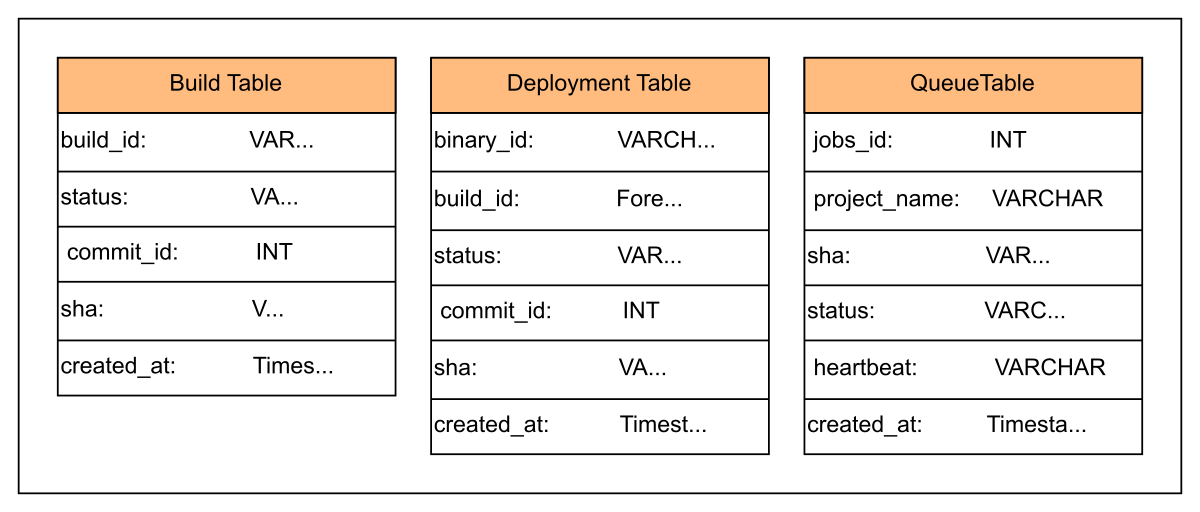
\includegraphics[width=0.5\textwidth]{Images/chapter_39/section_4940491583782912/6293252166516736.png}
 \caption{Storage schema for build, deployment, and the jobs in the queue}
\end{figure}

\begin{quote}
\textbf{Quiz:}
\textbf{Question 1:} How can we handle a scenario of the unexpected shutdown of a worker during the build process?
\textbf{Answer:} In the `QueueTable`, we have an attribute `Status`, which shows various phases of the job as shown below: Queued: When a job is placed in the queue, its status is changed to queued. Running: This shows a job is in the running phase and has been assigned to the code build service for generating artifacts. Failed: This status shows the job failed due to some technical errors. Completed: The job is completed, and its artifacts are stored in the blob store.

Canceled: The job is canceled. In addition to `status`, the table also includes a `heartbeat` attribute. This attribute stores periodic heartbeat signals sent by the worker processing the job. The worker updates this attribute regularly to show it is active. If the heartbeat is not updated within the expected timeframe, the system assumes the worker has failed. The job status is then reset to `Queued`, making it eligible for reassignment to another worker.
\end{quote}

After exploring the code deployment system's storage schema, let's focus on its detailed design, covering the internal components, their interactions, and the overall architecture.

\subsection{Detailed design}\label{uLpkxZEo00-VxcHILwBbE}
\\
The code deployment system comprises the following two phases:

\begin{itemize}
\item
\protect\phantomsection\label{7uWI7i6vfDitnpsIEKPDD}
The code-building phase
\item
\protect\phantomsection\label{Pt4m7lbgDFT21rF9QWjKF}
The code-deployment phase
\end{itemize}

\subsubsection{The code-building phase}\label{A3KR3kv6kUOS879LUAqMS}
\\
During the code-building phase, developers submit their code to a VCS such as GitHub. A CI system continuously monitors the repository for changes and is triggered whenever developers push updates or commit new code. Its primary purpose is to streamline the integration of changes from multiple contributors into a shared codebase. Beyond integration, the CI system also plays a crucial role in quality assurance by automatically running tests to catch potential issues early in the development cycle.
\\
The following illustration presents the components involved in the code-build system:\\

\begin{figure}[htbp]
 \centering
 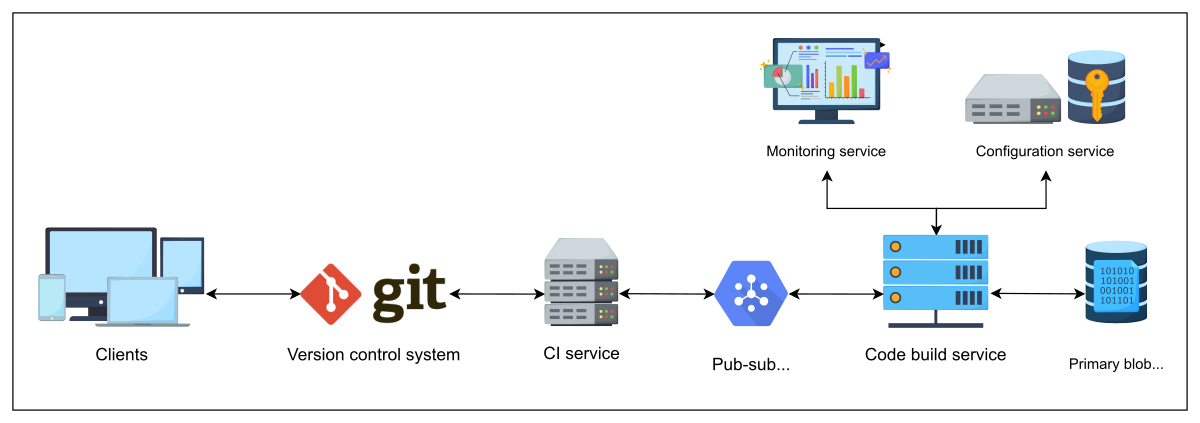
\includegraphics[width=0.5\textwidth]{Images/chapter_39/section_4940491583782912/5440861615554560.png}
 \caption{The code-building phase of the code deployment system}
\end{figure}

The CI system is also responsible for triggering the build automation process in which the code is submitted to the pub-sub system. The available code-build server retrieves the code from the pub-sub system and begins building it. The code-build servers form a cluster for building artifacts. Here , the code is checked for the latest changes, dependency installation, and required libraries, particularly from project configuration files such as \texttt{package.json} or \texttt{requirements.txt}. It also compiles, transpiles(Transpiling, short for "source-to-source compilation," is the process of taking source code written in one programming language and converting it into equivalent code in another language.), or builds the code into executable formats (binaries), depending on the technology stack, and stores it in the primary blob storage.
\\
Similarly, the build service may execute different tests, specifically unit and integration tests. The unit tests are executed to ensure that the code doesn't introduce regressions(Code regression refers to the unintended introduction of new bugs, errors, or issues into a software application that was previously functioning correctly. ). On the other hand, integration tests verify that the newly built code works correctly when interacting with other components.
\\
The configuration service manages the workers in the code-build service. It manages configuration information, synchronizes distributed processes, maintains distributed locks, and performs other related tasks. The primary focus of the configuration service is to provide reliability and availability while establishing coordination among the workers. Similarly , the monitoring service tracks the health, performance, and behavior of applications, systems, and networks. Monitoring services collect and analyze data from various sources, allowing administrators and teams to gain insights into the state of the code-build service.
\\
The workflow of the code-building phase is illustrated below:

\begin{figure}[htbp]
 \centering
 \begin{subfigure}[b]{0.48\textwidth}
 \centering
 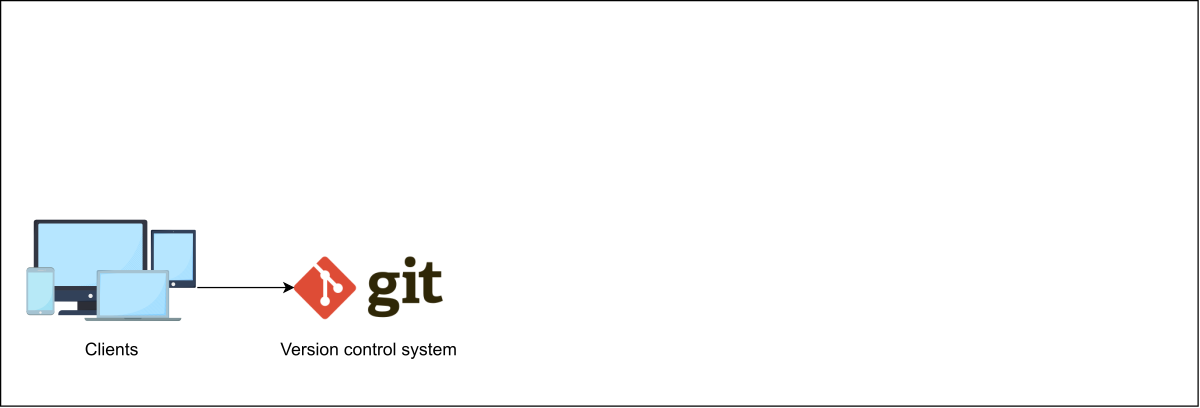
\includegraphics[width=\textwidth]{Images/chapter_39/section_4940491583782912/6013866154524672.png}
 \caption{Developers upload the code to a VCS such as GitHub}
 \end{subfigure}
 \hfill
 \begin{subfigure}[b]{0.48\textwidth}
 \centering
 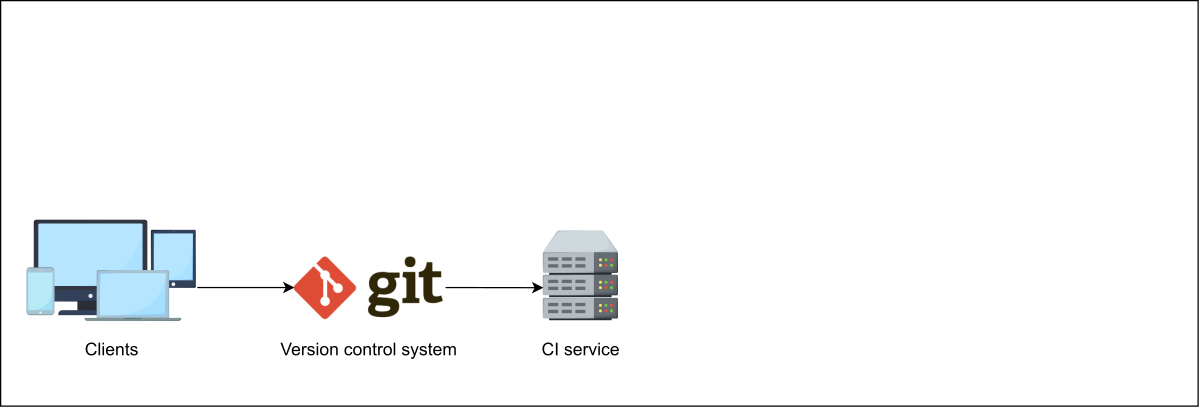
\includegraphics[width=\textwidth]{Images/chapter_39/section_4940491583782912/5136709949718528.png}
 \caption{The continuous integration system is activated whenever any changes are made to the VCS}
 \end{subfigure}
\end{figure}

\begin{figure}[htbp]
 \centering
 \begin{subfigure}[b]{0.48\textwidth}
 \centering
 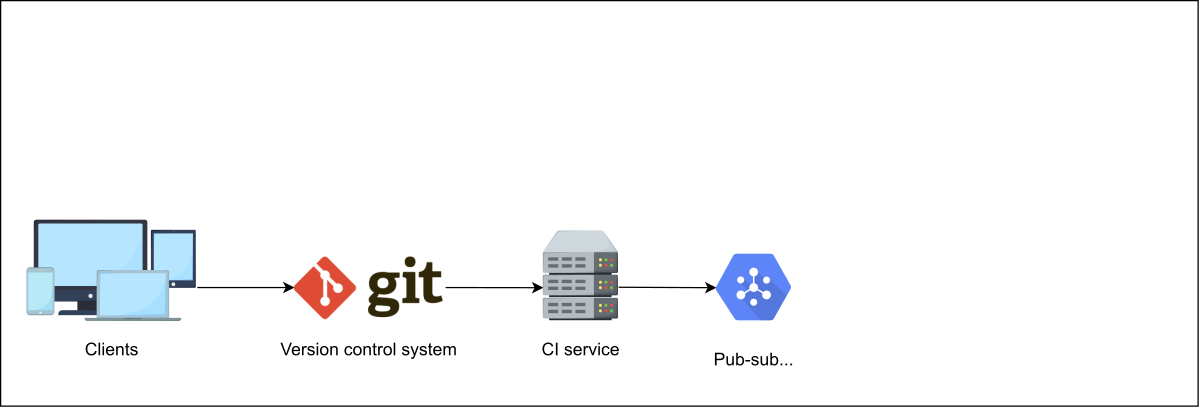
\includegraphics[width=\textwidth]{Images/chapter_39/section_4940491583782912/6274383636987904.png}
 \caption{The continuous integration system triggers the build process and the code is submitted to the pub-sub system}
 \end{subfigure}
 \hfill
 \begin{subfigure}[b]{0.48\textwidth}
 \centering
 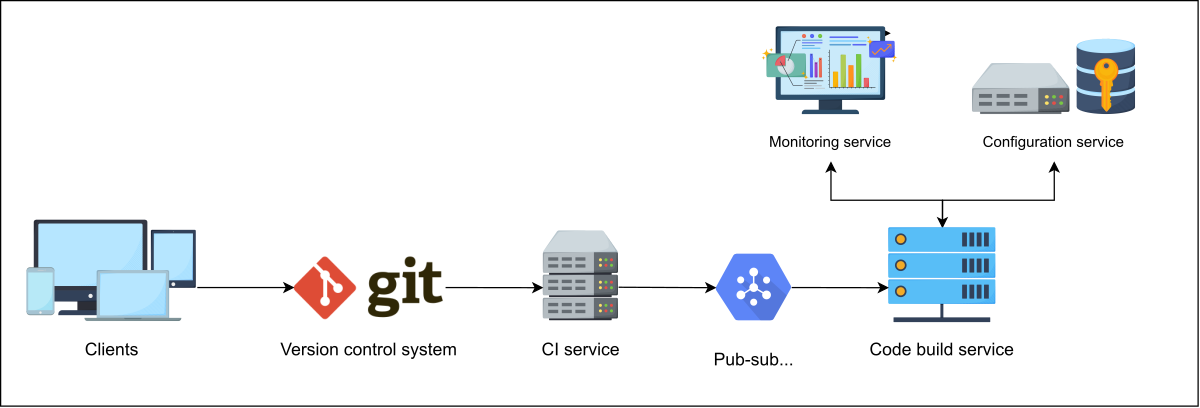
\includegraphics[width=\textwidth]{Images/chapter_39/section_4940491583782912/5663108389273600.png}
 \caption{The available workers take the code from the pub-sub system and start building it. The monitoring service keeps a check on the health of each worker, while the configuration service manages the workers in the build process}
 \end{subfigure}
\end{figure}

\begin{figure}[htbp]
 \centering
 \begin{subfigure}[b]{0.48\textwidth}
 \centering
 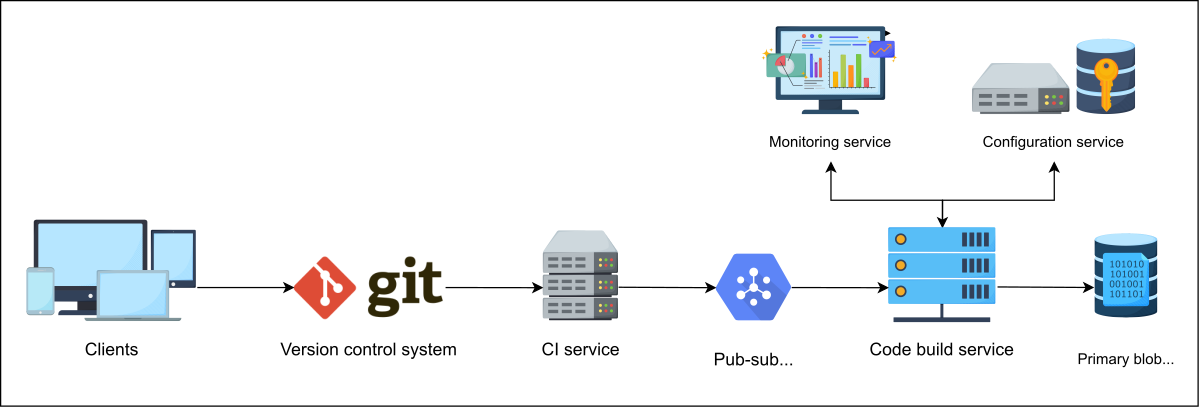
\includegraphics[width=\textwidth]{Images/chapter_39/section_4940491583782912/5771221306048512.png}
 \caption{When the code is built, it is stored in the primary blob storage for distribution to different regions when the deployment process is triggered}
 \end{subfigure}
\end{figure}

We've walked through how the code build process operates. Now , let's move on to the next stage of the deployment system and see what happens after the build is complete.

\subsubsection{Code deployment phase}\label{X8NSFcgbuuwU-3fn2NCfZ}
\\
Deploying code involves several phases beyond code-building, each ensuring that new changes are successfully integrated into production systems while minimizing disruptions.
\\
The following illustration shows the detailed design of the code deployment phase:\\
\strut \\

\begin{figure}[htbp]
 \centering
 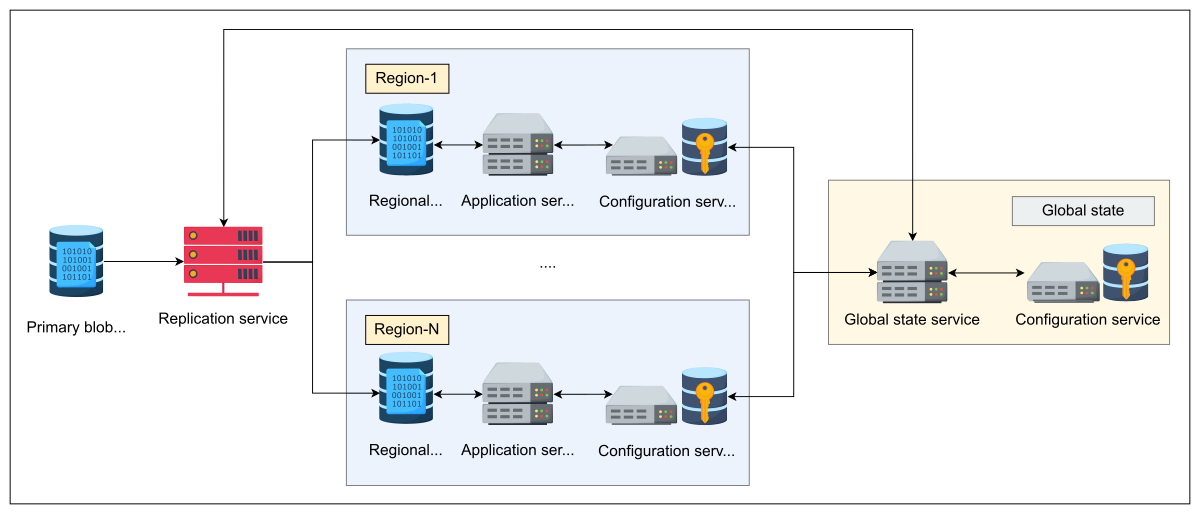
\includegraphics[width=0.5\textwidth]{Images/chapter_39/section_4940491583782912/6689442431369216.png}
 \caption{The deployment phase of the code deployment system}
\end{figure}

When the primary blob storage is updated with the binaries of the new code, the status in the queue is changed to \emph{Completed}. The replication service updates the regional blob storage with the new binary build. Earlier , we assumed that the minimum size of a single build is several gigabytes. Therefore, downloading the large file from the regional blob store to each machine over the network would take a considerable amount of time. We assume that the application servers in a region are connected via a peer-to-peer network. This will help decrease the binaries' downloading time to each machine.

\begin{quote}
\textbf{Quiz:}
\textbf{Question 1:} How does the performance differ when copying large binaries using the client-server paradigm as opposed to peer-to-peer (P2P)?
\textbf{Answer:} The difference in performance between copying big binaries using client-server and P2P is significant and depends on the architecture and network properties. In client-server architectures, a central server distributes binary files to multiple clients. The server becomes a bottleneck, particularly under high load, affecting overall performance.

In P2P architectures, the workload is distributed among multiple peers.

This means that transfers can be made in parallel and more efficiently.

P2P can take advantage of the upload or download capabilities of all the peers involved. This can lead to faster data transfer speeds, especially when the network has latency or bandwidth constraints.
\end{quote}

After the regional blob stores are populated with the latest binaries, the system updates a global state service that tracks deployment readiness across regions. This marks the binaries as ready for deployment throughout the system.
\\
To coordinate deployments, a key-value store keeps the desired version information. When a deployment is triggered, the global configuration is updated with the target version (e.g., \texttt{build:1.1}), as shown below:

\begin{lstlisting}[language=plaintext]
{ build_version: build:1.1
}
\end{lstlisting}

Regional configuration services continuously check the global state for updates. Once a new version is detected, each regional service notifies its local application servers to fetch the corresponding binaries from their regional blob store. The servers then download and install the new version, completing the deployment process.
\\
The configuration service in each region also ensures that code changes are seamlessly integrated into the production environment.

\begin{figure}[htbp]
 \centering
 \begin{subfigure}[b]{0.48\textwidth}
 \centering
 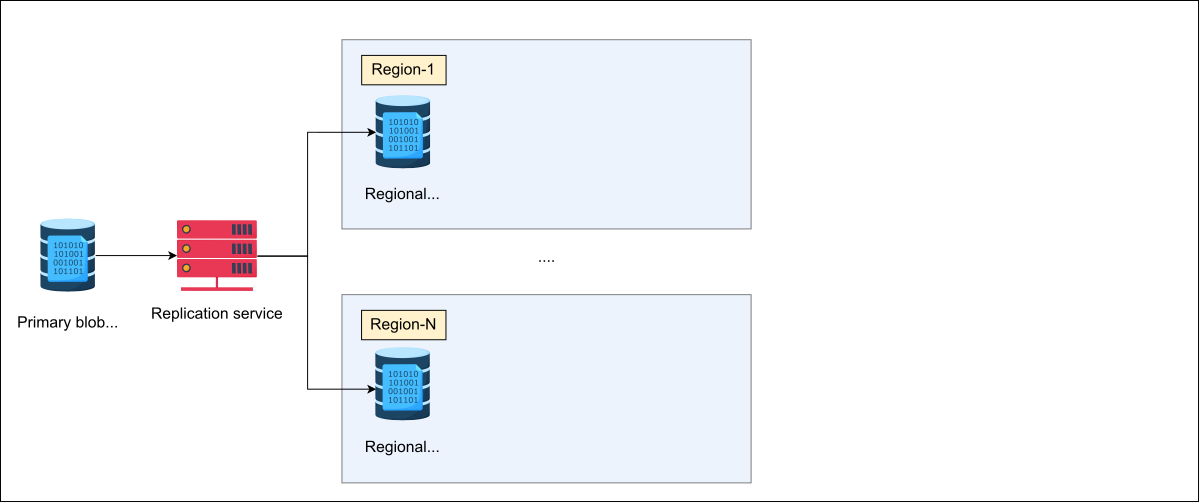
\includegraphics[width=\textwidth]{Images/chapter_39/section_4940491583782912/6317098227597312.png}
 \caption{When the code build status is changed to "Completed" the replication service updates the regional blob storage with the new build}
 \end{subfigure}
 \hfill
 \begin{subfigure}[b]{0.48\textwidth}
 \centering
 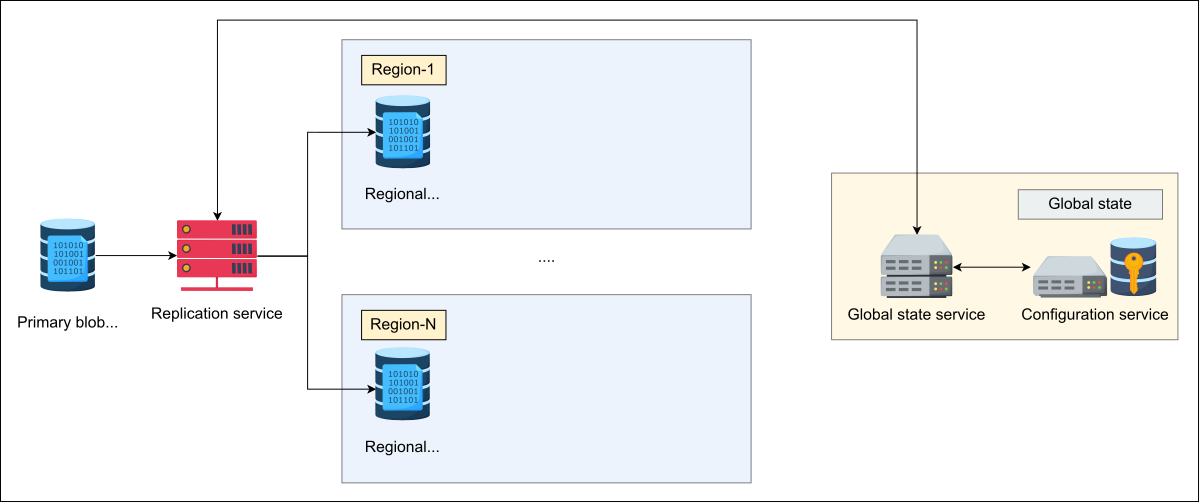
\includegraphics[width=\textwidth]{Images/chapter_39/section_4940491583782912/4544810983489536.png}
 \caption{The global state service is updated when the replication to each regional blob stores is completed. The binaries are now deployable}
 \end{subfigure}
\end{figure}

\begin{figure}[htbp]
 \centering
 \begin{subfigure}[b]{0.48\textwidth}
 \centering
 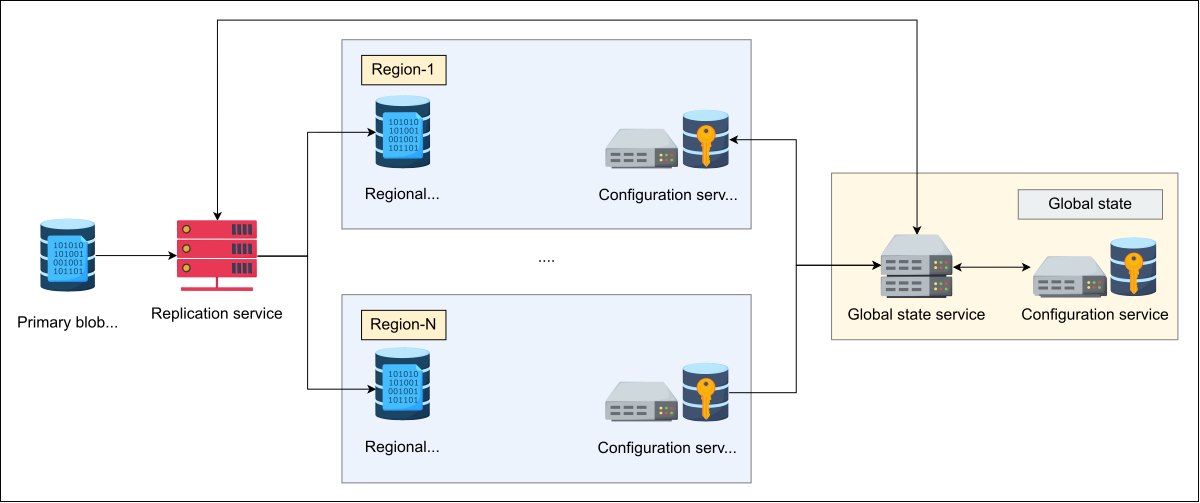
\includegraphics[width=\textwidth]{Images/chapter_39/section_4940491583782912/6512629230993408.png}
 \caption{Upon initiating the deploy command, the global state configuration service updates the regional configuration service}
 \end{subfigure}
 \hfill
 \begin{subfigure}[b]{0.48\textwidth}
 \centering
 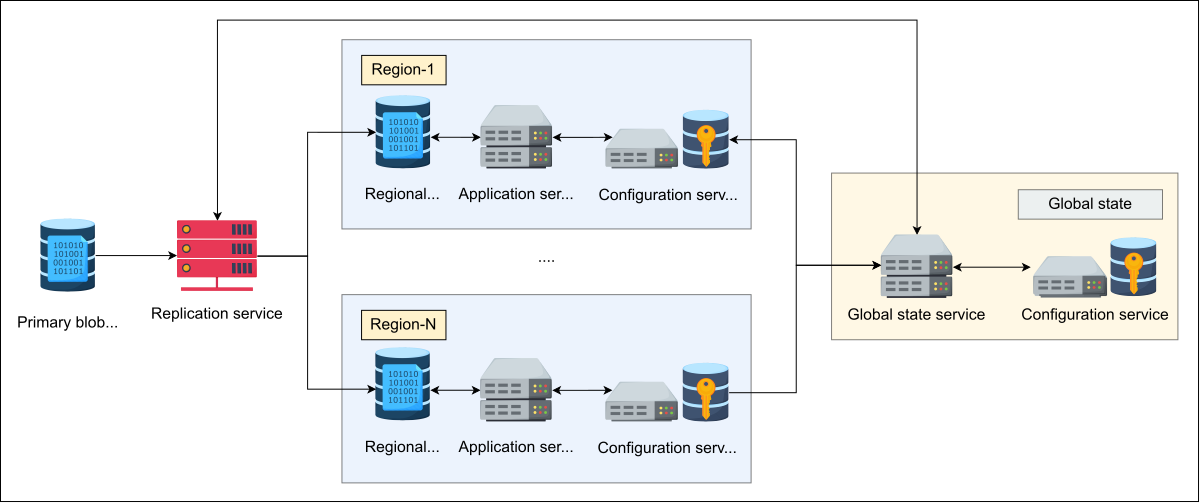
\includegraphics[width=\textwidth]{Images/chapter_39/section_4940491583782912/6564441636077568.png}
 \caption{The application servers continuously poll the regional configuration service for any changes. When any change is made to the configuration service, the application servers fetch the binaries from regional blob storage and install them}
 \end{subfigure}
\end{figure}

\subsection{Putting everything together}\label{uuLke91CkXpeb4_x6vETe}
\\
Let's put the build and deployment process together in the following figure. Once the code-build phase is completed, the replication service updates the regional blob storage with the newest build. Similarly , the global state configuration service is updated with the newest build version during deployment. The regional configuration service updates the newest build version and instructs the application server to download binaries from the updated regional blob storage. Once the download is completed to the regional blob storage, it is installed on each application server, and the application status is set to ``up''. This completes the deployment cycle.

\begin{figure}[htbp]
 \centering
 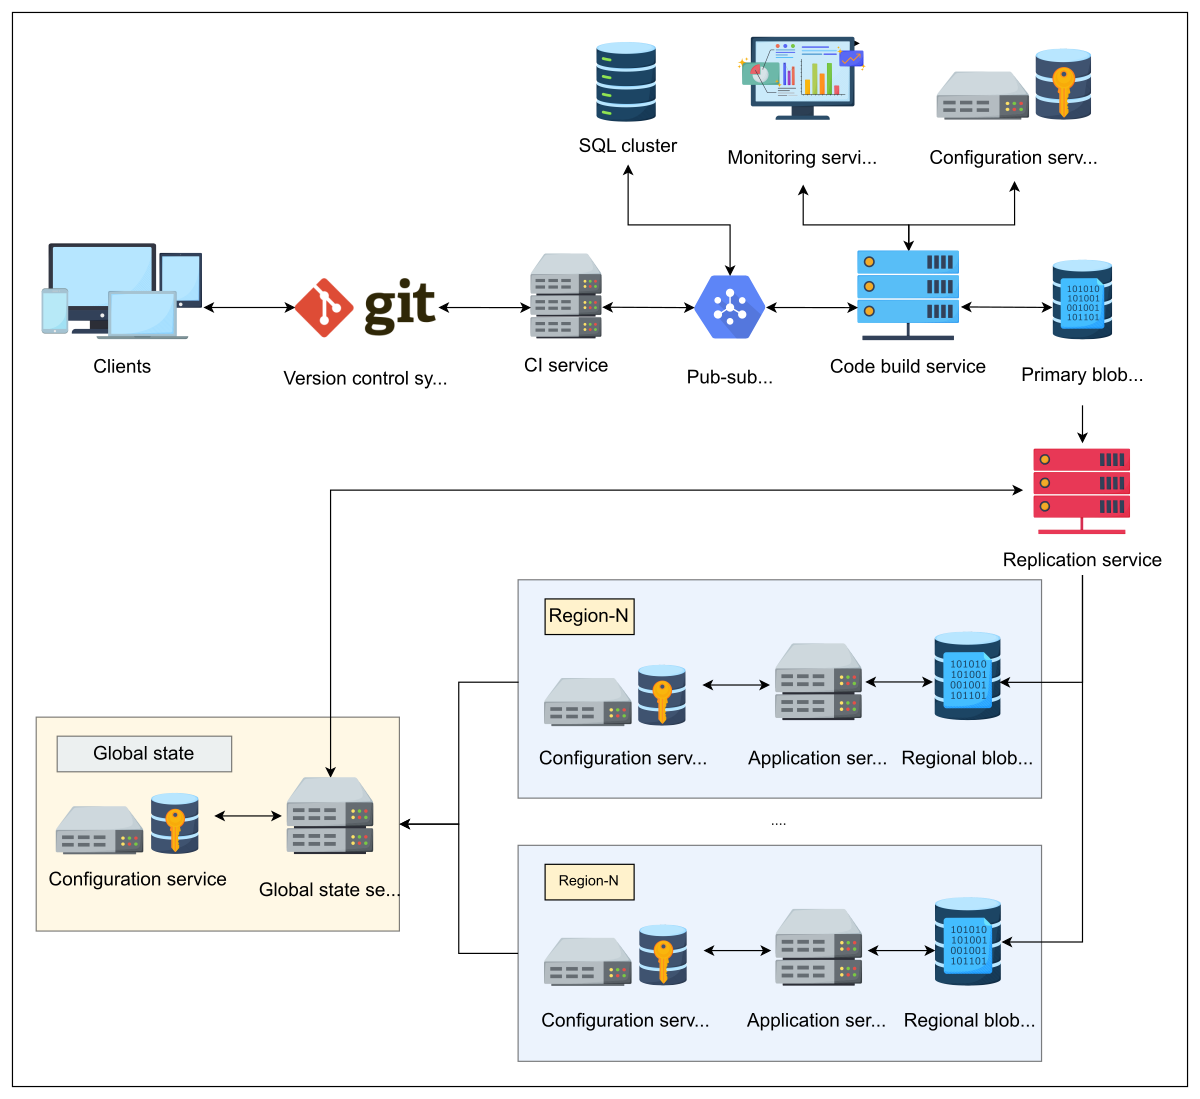
\includegraphics[width=0.5\textwidth]{Images/chapter_39/section_4940491583782912/6092685985054720.png}
 \caption{Detailed design of the code deployment system}
\end{figure}

\subsection{Requirements compliance}\label{Ufnp0FPyORgBKK8YMOicu}
\\
We will see how the proposed~design of the code deployment system satisfies both the functional and non-functional requirements essential for reliable, scalable, and observable software delivery across global infrastructure.

\subsubsection{Achieving functional requirements}\label{09PjGfV56nMUhxpY4yIPP}
\\
We will start by revisiting the functional requirements as mentioned in the previous lesson and examining how our~code deployment systemaddresses them:

\begin{table}[htbp]
\centering
\small
\adjustbox{max width=\textwidth}{
\begin{tabular}{|p{0.265\textwidth}|p{0.685\textwidth}|}
\hline
\textbf{Functional Requirements} & \textbf{Techniques} \\
\hline
\hline
Building code & \begin{itemize} \tightlist \item The~CI system~detects code changes and triggers the build process. \item The~code-build service, coordinated via the~pub-sub system, compiles and packages the code into binary artifacts (several GBs). \item The compiled output is stored in~primary blob storage to provide a durable and centralized location accessible by all deployment components \end{itemize} \\
\hline
Deploying code & \begin{itemize} \tightlist \item The replication service copies binaries from the primary to the regional blob storage. \item Application servers in each region download binaries via~peer-to-peer networks. \item Regional~configuration services~coordinate the update to local application servers. \end{itemize} \\
\hline
Version control integration & \begin{itemize} \tightlist \item The system integrates with~Git-based version control to enable the CI system to pull the latest changes from repositories for build and deployment. \end{itemize} \\
\hline
\ul{{}} Environment configuration & \begin{itemize} \tightlist \item A~central configuration service~maintains global and regional configuration states. \item Regional configuration services~fetch and apply environment-specific settings to application servers. \end{itemize} \\
\hline
Roll back & \begin{itemize} \tightlist \item The~configuration service~can update the deployment version (e.g.,~build:1.0) to a previous one tracked by the~global state service. \item Application servers can re-fetch and install older binaries from blob storage. \end{itemize} \\
\hline
Deploying monitoring & \begin{itemize} \tightlist \item The~monitoring service~tracks the health, status, and performance of the build and deployment pipeline, offering visibility into failures or delays. \end{itemize} \\
\hline
\end{tabular}
}
\end{table}

We have explored how the system design addresses functional requirements. Now let's see how the system meets non-functional requirements.

\subsubsection{Fulfilling non-functional requirements}\label{mQNsOD33083BoznPdi-7_}
\\
Beyond core functionality, a~code deployment system~must be fault-tolerant, scalable, and secure to support continuous delivery at a global scale. The table below summarizes how the design meets these critical non-functional requirements:

\begin{table}[htbp]
\centering
\small
\adjustbox{max width=\textwidth}{
\begin{tabular}{|p{0.239\textwidth}|p{0.711\textwidth}|}
\hline
\textbf{Non-functional Requirements} & \textbf{Techniques} \\
\hline
\hline
Availability & \begin{itemize} \tightlist \item The configuration service enables automated failover by rerouting build requests to backups. \item Redundancy is ensured with duplicated servers, databases, and load balancers. \end{itemize} \\
\hline
Fault tolerance & \begin{itemize} \tightlist \item The monitoring system checks system health and notifies administrators. \item Workers regularly send heartbeats through the pub-sub system, recorded in an SQL database; if one is missed, the task is reassigned to an available worker. \end{itemize} \\
\hline
Performance & \begin{itemize} \tightlist \item Builds are executed asynchronously to avoid blocking. \item Binaries are distributed across regions. \item Peer-to-peer network within each region enables fast replication. \end{itemize} \\
\hline
Scalability & \begin{itemize} \tightlist \item Queue service auto-scales with build request volume. \item Configuration service deploys more servers as needed. \item System resources dynamically adjust based on load. \end{itemize} \\
\hline
Security & \begin{itemize} \tightlist \item Multi-factor authentication (MFA) and OAuth are enforced. \item Data is encrypted at rest and in transit. \item Secure coding practices, firewalls, and intrusion detection are used. \item IAM service handles access control and credential management and enforces the least privilege. \end{itemize} \\
\hline
\end{tabular}
}
\end{table}

We've explored the non-functional requirements and the techniques used to achieve them. Let's test our understanding with a quiz.

\subsection*{Quiz}
\vspace{0.3cm}
\noindent
\textbf{Question 1:} What mechanism is established to ensure system availability during the build phase?
\\[0.2cm]
\begin{itemize}
 \item OAuth authentication
 \item \textbf{[CORRECT]} Redundancy through duplicated elements
\\[0.1cm]
\textit{Explanation:} 
Redundancy of resources enhances the system's availability. If one component fails, the other is on standby to provide the desired services.
 \item Elastic resources management
 \item Blue-green deployment strategy
\end{itemize}
\vspace{0.3cm}
\noindent
\textbf{Question 2:} How does the queue service handle scalability during the build phase?
\\[0.2cm]
\begin{itemize}
 \item Through OAuth authentication
 \item \textbf{[CORRECT]} Through elastic resources and auto-scaling
\\[0.1cm]
\textit{Explanation:} 
Elastic resource management adds or removes resources based on the current load, which enhances the scalability of the system.
 \item Through the blue-green deployment strategy
 \item Through intrusion detection and firewalls
\end{itemize}
\vspace{0.3cm}
\noindent
\textbf{Question 3:} How does the code deployment system address the challenge of a failing worker during the build phase for fault tolerance?
\\[0.2cm]
\begin{itemize}
 \item Multi-factor authentication (MFA)
 \item Auto-scaling the configuration service
 \item Regular vulnerability management
 \item \textbf{[CORRECT]} Heartbeat mechanism and job reassignment
\\[0.1cm]
\textit{Explanation:} 
The heartbeat mechanism ensures a worker is up and performing the build process. If a worker fails to send a heartbeat in the designated time, it is considered failed, and the build job is assigned to another worker.
\end{itemize}

We've seen the detailed design of the code deployment system. Now, let's explore how a deployment strategy impacts the System Design:

\subsection{Impact of deployment strategies on the CDS}\label{Fw-m_jnbeo8WduFajSqk0}
\\
The deployment strategy adopted in a code deployment system (CDS) plays a significant role in shaping its architectural decisions. In our proposed design, we rely on a~basic deployment strategy, which is flexible and straightforward to implement. While simple, this strategy requires~careful handling of version consistency and rollback mechanisms~to ensure reliability during the rollout process.
\\
Different deployment strategies, such as~blue-green~or~canary deployments, have distinct requirements that must be accommodated within the System's Design. For instance, a blue-green deployment necessitates the creation of duplicate environments, while a canary deployment demands mechanisms to roll out changes to a subset of users gradually.
\\
The choice of deployment strategy can significantly impact requirements such as redundancy, load balancing, version management, and monitoring mechanisms. Therefore, a code deployment system should be designed to be flexible and modular. It should support various strategies tailored to project needs, ensuring performance, reliability, and scalability.
\\
What trade-offs exist between performance and reliability when implementing a blue-green deployment?
\\
Use the AI assessment widget below to submit your solution and get an interactive response.

\textbf{Question:}

Performance vs. reliability 

\textbf{Reference Answer:}

A blue-green deployment improves reliability by allowing instant rollback and zero-downtime releases, but it introduces performance trade-offs because you must run two full production environments simultaneously, which doubles infrastructure usage and can strain resources. Traffic switching also risks cache cold-starts, uneven load distribution, or momentary latency spikes as the new environment warms up. In short, you gain safer, more reliable releases at the cost of higher resource consumption and potential short-term performance dips.

\subsection{Conclusion}\label{DOd6KpBDbNVWEhs8gDFqK}
\\
Designing a scalable and resilient code deployment system depends on various organizational and architectural decisions. This chapter presents an approach to building a flexible deployment system, focusing on the code-building process and a basic deployment strategy. Since deployment can follow multiple strategies, choosing a specific one can significantly influence the system's overall design. Supporting components such as VCS and CI are acknowledged but not explored in depth due to their inherent complexity. Finally , the chapter discusses various methods for meeting requirements and examines how different deployment strategies affect the overall design of the code deployment system.

% End of section content